% !TEX TS-program = pdflatex
% !TEX encoding = UTF-8 Unicode

% This is a simple template for a LaTeX document using the "article" class.
% See "book", "report", "letter" for other types of document.

%\documentclass[12pt]{article} % use larger type; default would be 10pt
%\documentclass[1p]{elsarticle} 
%\documentclass[preprint,12pt]{elsarticle}
\documentclass[final,1p]{elsarticle}
%\usepackage[utf8]{inputenc} % set input encoding (not needed with XeLaTeX)

%%% Examples of Article customizations
% These packages are optional, depending whether you want the features they provide.
% See the LaTeX Companion or other references for full information.

%%% PAGE DIMENSIONS
%\usepackage{geometry} % to change the page dimensions
%\geometry{a4paper} % or letterpaper (US) or a5paper or....
% \geometry{margin=2in} % for example, change the margins to 2 inches all round
% \geometry{landscape} % set up the page for landscape
%   read geometry.pdf for detailed page layout information
%\usepackage{}
\newcommand\aap{{A\&A}}%
          % Astronomy and Astrophysics
\newcommand\apj{{ApJ}}
\newcommand\apjl{{ApJL}}
\newcommand\jcp{{J. Comput. Phys.}}
\newcommand\solphys{{Sol. Phys.}}

\usepackage{graphicx} % support the \includegraphics command and options
%\usepackage[longnamesfirst,nonamebreak]{natbib}
% \usepackage[parfill]{parskip} % Activate to begin paragraphs with an empty line rather than an indent

%%% PACKAGES
%\usepackage{booktabs} % for much better looking tables
%\usepackage{array} % for better arrays (eg matrices) in maths
%\usepackage{paralist} % very flexible & customisable lists (eg. enumerate/itemize, etc.)
%\usepackage{verbatim} % adds environment for commenting out blocks of text & for better verbatim
%\usepackage{subfig} % make it possible to include more than one captioned figure/table in a single float
% These packages are all incorporated in the memoir class to one degree or another...
\usepackage{amsmath}
\usepackage{amssymb}
\usepackage{hyperref}
%%% HEADERS & FOOTERS
%\usepackage{fancyhdr} % This should be set AFTER setting up the page geometry
%\pagestyle{fancy} % options: empty , plain , fancy
%\renewcommand{\headrulewidth}{0pt} % customise the layout...
%\lhead{}\chead{}\rhead{}
%\lfoot{}\cfoot{\thepage}\rfoot{}

%%% SECTION TITLE APPEARANCE
%\usepackage{sectsty}
%\allsectionsfont{\sffamily\mdseries\upshape} % (See the fntguide.pdf for font help)
% (This matches ConTeXt defaults)

%%% ToC (table of contents) APPEARANCE
%\usepackage[nottoc,notlof,notlot]{tocbibind} % Put the bibliography in the ToC
%\usepackage[titles,subfigure]{tocloft} % Alter the style of the Table of Contents
%\renewcommand{\cftsecfont}{\rmfamily\mdseries\upshape}
%\renewcommand{\cftsecpagefont}{\rmfamily\mdseries\upshape} % No bold!

%%% END Article customizations

%%% The "real" document content comes below...
\begin{document}


\title{Simulations of the Dynamics Generated by Solar Global  Oscillating Eigenmodes Generated in the Solar Atmosphere}
\author[swat,cics]{M.K.Griffiths \corref{cor1}}
\author[acse]{V.Fedun}
\author[swat]{R.Erd\'{e}lyi}
%\author[cics]{D.Savas }
%\author{M.K.Griffiths\corref{cor1}\fnref{fn1},V.Fedun, D.Savas\tnoteref{tno2} and  R.Erd\'{e}lyi}
%\date{} % Activate to display a given date or no date (if empty),
         % otherwise the current date is printed 
\address[swat]{Solar Physics and Space Plasma Research Centre ($SP^{2}RC$), School of Mathematics and Statistics, University of Sheffield, Hicks Building, Hounsfield Road, S7 3RH, UK}
\address[cics]{Corporate Information and Computing Services, The University of Sheffield, 10-12 Brunswick Street, Sheffield, S10 2FN, UK}
\address[acse]{Department of Automatic Control and Systems Engineering, The University of Sheffield, Mappin Street, Sheffield, S1 3JD, UK}
%\fnref{<label(s)>}
%\tnotetext[<label>]{<title note text>}
%\cortext[cor1]{email: m.griffiths@sheffield.ac.uk}
\cortext[cor1]{Corresponding author at: Corporate Information and Computing Services, The University of Sheffield, 10-12 Brunswick Street, Sheffield, S10 2FN, UK. \linebreak e-mail address: m.griffiths@sheffield.ac.uk}

\begin{abstract}
The solar atmosphere exhibits a diverse range of wave phenomena one of the earliest to be discovered was the five minute oscillation, the p-mode. The solar p modes are generated by global resonant oscillations and turbulent motions just beneath the photosphere. The resulting propagation of this wave energy into the solar atmosphere may be used as a diagnostic tool to predict some of the physical characteristics of the  suns atmospheric layers. We report on a study of synthetic photospheric oscillations for a magnetic field free  model of the quiet sun

 The objective of this paper is to investigate the dynamics in the solar atmosphere which are generated by solar global eigenmodes of oscillation and to the understand the leakage mechanisms of the five minute global oscillations into the atmosphere. Understand the conditions under which chromospheric dynamics evolve as a result of the 5 minute global oscillations - (spicules, waves).  The main idea of performed simulations is to understand how energy supplied by various wave modes (the supplied energy is same for all of them) is redistributed in the atmosphere. Establish a link between signals at the photospheric levels and those at Coronal levels and shed light on the mechanisms leading to ubiquitous intensity oscillations in the solar atmosphere. The drivers in these simulations are different from our previous numerical experiments i.e. here we perturbed the whole bottom boundary.

 We report on a series of hydrodynamic simulations of a realistic model of the solar atmosphere with a driver located at 0.5Mm above the temperature minimum. With the objective of recreating atmospheric motions generated by global resonant oscillation the driver is spatially structured and is extended in a sinusoidal profile arcoss the base of the computational model.  To carry out the simulations, we employed our the MHD code SMAUG (Sheffield MHD Accelerated Using GPUs). A combination of the VALIIIC and McWhirter solar atmospheres and coronal density profiles were used as the background equilibrium
model in the simulations. Vertical and horizontal harmonic sources, located at the footpoint region of the open magnetic flux tube, are incorporated in the calculations, to excite oscillations in the domain of interest.

Our results show that the amount of energy propagated into the solar atmosphere is consistent with a model of solar global oscillations described using the Klein-Gordon equation. Our results indicate a power law behaviour consistent with that of recent observational results obtained using the Atmospheric Imaging Assembly of the Solar dynamics observatory (SDO AIA)  \cite{Ireland2014}.

Our results demonstrate the conversion of modes with a period of 30s to a mode with a period of 180s, demonstrating that the Chromosphere is a source of 180s modes. The results inidicate a shift in frequency arising from interference between the driven waves and reflections from the transition layer.
\end{abstract}

\begin{keyword}
magnetohydrodynamics (MHD); oscillations; MHD waves; solar atmosphere
\end{keyword}
\maketitle

%\maketitle



\section{Introduction}
\setcounter{equation}{0}
The solar atmosphere exhibits a diverse range of wave phenomena. The first Observations of oscillatory behaviour reported vertical motions on the solar surface with an amplitude of 300-400m/s with a period of 296s observations of Ca K band \cite{Leighton1960}. These ubiquitous oscillations are referred to as the p-modes.
These motions were attributed to standing acoustic waves in the solar interior \cite{Ulrich1970}. It was reported that the vertical wavelength is comparable to the horizontal wavelength and is roughly 1000-5000km \cite{Leibacher1971}.  The main restoring force for these modes of oscillation is the pressure, the 5 minute oscillation is the main manifestation of these modes. The detection of oscillations in the apparent solar diameter (Hill et al 1976, Brown et al 1978) was one of the first suggestions of the truly global oscillations of the sun.  The work of Christensen-Dalsgaard modelling solar oscillations on the basis of the solar structure provided spectra consistent with those of Hill, this was the start of helioseismology. The perturbation of a dynamical system such as the gravitationally stratified solar atmosphere results in the occurence of eigen-oscillations, these oscillations resulting from the internal interactions of the system. A model for understanding these oscillations can be understood from the normal mode solutions of the gravitating  hydrodynamic slab in ideal MHD (Goedbloed & Poets). The solar p modes are generated by global resonant oscillations, periodic  and turbulent motions just beneath the photosphere.  These resonant modes are reflected at the surface by the steep change in density. The increase of the sound speed causes refraction.   The resulting propagation of this wave energy into the solar atmosphere may be used as a diagnostic tool to predict the physical characteristics of the  suns atmospheric layers. We report on a series of hydrodynamical simulations modelling a realistic solar atmosphere using a driver located at the temperature minimum, the driver is extended in a sinusoidal profile arcoss the base of the computational model.  The objectives of this work is to recreate the atmospheric motions generated by the global resonant oscillation, to  understand how the energy provided by different modes of oscillation are redistributed in the solar atmosphere and to shed light on the mechanisms which lead to ubiquitous intensity oscillations in the solar atmosphere.   

\section{Observations and Computational Studies Oscillations in the Solar Atmosphere}

There is a significant body of work reporting on observational, theoretical and computational studies of p-mode phenomena. This work generally describes mechanisms for the propagation of energy into the Chromosphere, into the Solar Corona or between the transition region and the Corona. We briefly summarise some of this work here. 

The growing field of coronal seismology uses the observed solar atmospheric wave modes to determine the physical characterisitcs of the solar atmosphere. This in turn requires a thorough understanding of the physics of the solar atmosphere. Although there is overwhelming evidence for photospheric 5 minute p-modes and 3 minute Chromospheric modes, the detection and characterisation of oscillatory phenomena in the corona are rare and difficult to detect. This makes the solution of the coronalheating problem more challenging. However, since the advent of Coronal Seismology \cite{Roberts1984} \cite{DeMoortel2005} many spaced based high resolution systems (SOHO, TRACE, SDO) have provided evidence for wave like perturbations in the solar atmosphere.
The work of \cite{Erdelyi2015} provides a detailed study of intensity oscillations in the solar atmosphere. Using SDO/AIA data they study image sequences at somlar minimum and maximum for diffrent solar regions e.g. active regions, quiet sun and a coronal hole. They consider a lower coronal channel, hot coronal channel and a cooler coronal channel. The study revealed strong 3-5 minute oscillations in all channels and included some longer period modes. The results indicated that diffrences my arise when the size of the area of observation is changed.The ubiquity of the observed 3 and 5 minute oscillations in all channels and regions is an indication of a global excitation mechanism.

 Imagery from SDO $171\AA$ and $193\AA$ was used by \cite{Ireland2014} to compute the Fourier power spectra in the Corona. Studying four regions of the solar atmosphere with different characteristics, they found that the distribution obeys a power law at low frequencies and possesses a flat distribution at high frequencies. This contrasts with the idea of a Gaussian noise distribution and a long time scale background. The implication is that this is the result of solar atmospheric heating from everywhere by small energy deposition events. It is expected that further measurements will constrain computational models. 

Evidence for the upward propagation of acoustic wave with increasing amplitude has been demonstrated through a studies of variation in the intensities of Chromospheric lines for example the Ca lines at 854nm \cite{Beck2012}. Although the observed variations are unlikely to provide temperature rises observed in the Chromosphere they are a clear indication of the increase in dynamical activity from the photosphere to the chromosphere. The analysis of observations from the Observatorio del Teide/Tenerife by Bello et al \cite{Bello2009}, find that at a height of 250km there is an acoustic energy flux of $3000W/m^2$  $2/3$ of this energy is propagated by waves in the frequency range 5-10mHz, the remaining third is carried by waves in the frequency range 10-20mHz. Waves with frequencies greater than the acoustic cut-off of 190s can contribute to the heating of the solar chromosphere. Reporting on measurements from the the Fe I $5434{\AA}$ \cite{Bello2010A} detect waves with periods down to $40s$. For periods below the cutoff of $190s$ 40% of wave detections are above granules the remaining 60% are above the intergranules. The reported best estimate of the energy flux above granules is around $3000W/m^{2}$ whilst above the intergranules it is around $955W/m^2$. Most of the acoustic flux is found between $110s$ and $193s$.

Using the IMAX instrument on the sunrise observatory, Roth et al  \cite{Roth2010}  reported evidence for the excitation of solar acoustic oscillations excited by turbulent flows  in the dark intergranular lanes.  Individual sunquakes with epicenters near the solar surface and located in the intergranular lanes, are assumed to feed continuously energy into the resonant p-modes of the Sun and provide sources for acoustic oscillations. Roth presents wavefronts rippling near a granule and oriented along the direction of the intergranular lane. Using simultaneous observations of the Na and K lines with Doppler measurements Jefferies et al \cite{Jefferies2006} show that inclined magnetic field lines provide portals along which magnetoacoustic energy can propagate at the intergranular boundaries.

There is a large body of computational work already undertaken Among others the following \cite{Fedun2009} et al study the Oscillatory Response of the 3D Solar Atmosphere to the Leakage of Photospheric Motion results are discussed in detail: i) High-frequency waves are shown to propagate from the lower atmosphere across the transition region, experiencing relatively low reflection, and transmitting most of their energy into the corona; ii) the thin transition region becomes a wave guide for horizontally propagating surface waves for a wide range of driver periods, and particularly at those periods that support chromospheric standing waves; iii) the magnetic field acts as a waveguide for both high- and low-frequency waves originating from the photosphere and propagating through the transition region into the solar corona.


Previous work has considered either point source drivers with a gaussian velocity distribution Other work e.g. by K. Murawski, T.V. Zaqarashvili (2010) \cite{Murawski2010} has demontrated that The numerical simulations show that the strong initial pulse may lead to the quasi periodic rising of chromospheric material into the lower corona in the form of spicules Khomenko and SantaMaria \cite{Khomenko2012}. Kalkofen \cite{Kalkofen2010} considered the propagation of acoustic modes in a stratified hydrodynamical model of the solar atmosphere, they employed a cylindrically symmetric driver with a diameter of approximately $1Mm$. They conclude that for driving regions of sizes smaller than the atmospheric scale height they are able to reproduce expansion waves which are characteristic of Chromospheric bright points. With a weak horizontal magnetic field, the physics within the interior of supergranulation cells \cite{Lites2008} is suitably simple for undertaking hydrodynamic modelling. The objective of the work presented here  is to characterise the dynamics generated by these solar global oscillating eigenmodes generated in the solar atmosphere.  These modes ARE some sort of global eigenmodes. The coherence length of eigenoscillations at the photoshphere is about a few Mm, and the power peaks at around 3-5 mins. 



%__________________________________________________________________



\section{Numerical Computation Methods}
To model the time-dependent evolution of photospheric oscillations in the solar atmosphere  we solve the 3D ideal MHD equations.   The 3D numerical simulations described here here were undertaken using SMAUG, the GPU implementation of the Sheffield Advanced Code (SAC)\cite{Griffiths2015}\cite{Shelyag2008}. SAC and SMAUG are numerical MHD solvers allowing the simulation of a variety of physical processes in magnetised plasmas.  With the upper boundary of our model in the Solar Corona and the lower boundary in the photosphere the SMAUG code is well suited for modelling the leakage of wave energy from the photopshere, through the transition zone and into the photosphere. With open boundary conditions for the lower and upper boundaries it is possible to model wave propagation for time scales characterised by the 5 minute p-mode induced oscillations. The general system of MHD equations are
\begin{equation}\label{eqdens}
{{\partial \rho}\over{\partial t}}+\nabla\cdot\left( {\bf v}\rho\right)=0,
\end{equation}

\begin{equation}\label{eqmom}
{{\partial ( \rho {\bf v})}\over{\partial t}}+\nabla\cdot\left( {\bf v}\rho {\bf v}-{\bf B B}\right)+\nabla p_t=\rho{\bf g},
\end{equation}

\begin{equation}\label{eqe}
{{\partial e}\over{\partial t}}+\nabla.\left({\bf v}e-{\bf B B}\cdot{\bf v}+{\bf v}p_{t}\right)+\nabla p_t=\rho{\bf g}\cdot{\bf v},
\end{equation}

\begin{equation}\label{eqb}
{{\partial{\bf B}}\over{\partial t}} +\nabla \cdot\left(  {\bf vB}-{\bf Bv}\right)=0.
\end{equation}

In these equations $\rho$ is the mass density, $  \bf { v} $ is the velocity,   $ \bf B$ is the magnetic field, $\it{e}$ is the energy density, $p_{t}$ is the total pressure and $\bf g$ is the gravitatioanl acceleration vector.

The total pressure $p_{t}$ is written as
\begin{equation}\label{eqpt}
p_{t}=p_{k}+{{\bf B}^{2}\over{2}},
\end{equation}
where $p_k$ is the kinetic pressure given by
\begin{equation}\label{eqpk}
p_{k}=(\gamma - 1)( e-{{\rho \bf v }^{2}\over{2}}-  {{\bf B}^{2}\over{2}} ).
\end{equation}

The equations \eqref{eqdens} to \eqref{eqpk} are applicable to an ideal compressible plasma. The SAC code is based on perturbed versions of these equations, thus the variables $\rho $, $e$ and  $\bf B$ are expressed in terms of perturbed and background quantities as
\begin{equation}
\rho = \tilde{\rho}+\rho _{b},
\end{equation}
\begin{equation}
e = \tilde{e}+e _{b},
\end{equation}
\begin{equation}
\bf B = \tilde{\bf B}+{\bf B}_{\it{b}}.
\end{equation}
where $\tilde{\rho}$ is the  perturbed density,  $\tilde{e}$ is the perturbed energy and $\tilde{\bf B}$  is the perturbed magnetic field. The background quantities with a subscript $\it{b}$ do not change in time, as we assume a magneto-hydrostatic equilibrium of the background plasma which may have a gravitational field present, denoted by $\bf g$. Hyper-diffusion and hyper-resistivity \cite{Caunt2001}
are implemented to achieve numerical stability of the computed solution of the MHD equations.  The full set of MHD equations, including the hyper-diffusion source terms are given in \cite{Griffiths2015}\cite{Shelyag2008}.









%__________________________________________________________________


\section{Solar Atmospheric Model}
In order oscillatory phenomena in the Solar Corona a physically representative model of the solar atmosphere is needed. An option is the use of a parametrisation of the tempearture of the solar atmosphere which may be a smoothed step function profile  \cite{Murawski2010}. Results have demonstrated the need for observationally derived semi-emprical models of the solar atmosphere. There is much discussion about model validity and the work undertaken to demonstrate the reliability of the assumptions used to construct realistic models of the solar chromosphere \cite{Carlsson1995}, \cite{Kalkofen2012}. The contention arises from the dynamical nature of the solar chromosphere for example local dynamo action has been suggested as a mechanism of Joule heating in the solar chromosphere \cite{Leenaarts2011}. The model atmosphere employed here is an observationally derived semi-empirical representation of the quiet sun. With the fundamental assumption of hydrostatic equilibrium a model of the chromosphere in equilibrium is constructed using the VALIIc model \cite{Vernazza1981}. For the region of the solar atmosphere above 2.5Mm the results of the energy balance model of solar coronal heating has been used  \cite{McWhirter1975}, this model includes an acoustic contribution comparable to the hydrostatic pressure.



%FIGURE 1 here caption:Temperature and Density Profiles Used for the Model Atmosphere.\\

\begin{figure*}[h]
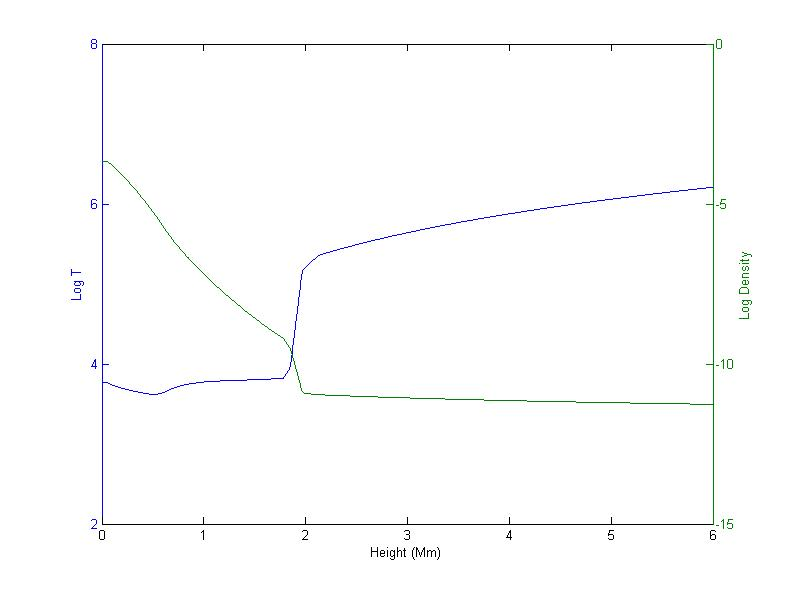
\includegraphics[scale=0.5]{images/VAL3C_rho_temp_fig2.jpg}
\caption{Temperature and Density Profiles Used for the Model Atmosphere. }
\end{figure*}



%FIGURE 2 here caption:Cut of Frequency at Different Heights in the Model  Solar Atmosphere..\\

\begin{figure*}[h]\label{cutofffrequency_fig4}
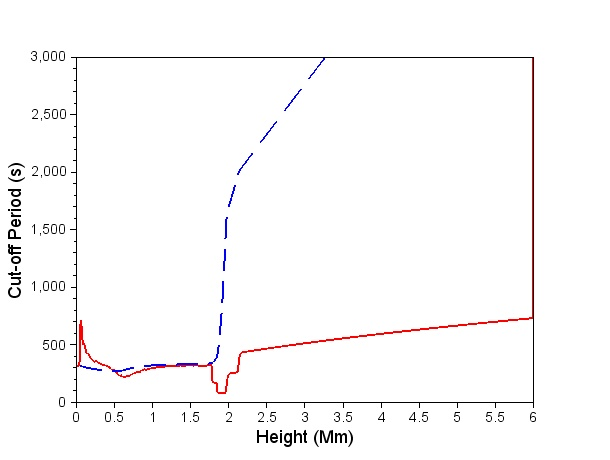
\includegraphics[scale=0.7]{images/cutofffrequency_fig4.jpg}
\caption{Cut of Frequency at Different Heights in the Model  Solar Atmosphere. }
\end{figure*}




%__________________________________________________________________

\section{Numerical Drivers for p-Mode Oscillations}
The overview of observational studies identified a range of physical phenomena resulting in oscillatory behaviour and delivering energy into the solar atmosphere.  The results presented here extend earlier work undertaken by  \cite{Malins2007A}, for their study point drivers were used to represent periodic buffeting or turbulent motions in the photosphere. The point driver is described by \eqref{eqpointdriver} has width  $\Delta x$ of $4Mm$ and width $\Delta z$  of $4km$ applied to a 2D model of the realistic solar atmosphere. The results of the study demosnstrated surface wave phenomena and structures in the transition zone and highlighted the characteristics of the oscillatory phenomena as a result of frequency cutoffs induced by the stratified solar atmosphere. 

\begin{equation}\label{eqpointdriver}
V_{z}=A \sin{\left({2\pi t}\over{T_s} \right)  }  \exp{\left( -{(x-x_0)^{2}}\over{\Delta x^{2}} \right) } \exp{\left( -{(z-z_0)^{2}}\over{\Delta z^{2}} \right) },
\end{equation}

For this study the model requires a driver mimicing the solar global oscillations.    In the real Sun, photospheric p-mode oscillations have a horizontal wavelength and coherence. Here, these excitations are represented with a vertical velocity driver located at the photosphere, this acoustic p-mode driver excites waves which propagate into a realisitc 3D model of the Solar atmosphere. Drivers representing different modes are considered, for example  an extended driver with a sinusoidal dependence and a wavelength of 8 Mm applied along the middle of the base of a computational domain of dimension 4Mm represents  a “fundamental mode”. A driver with wavelength 4 Mm applied the same way represents the “first harmonic”.  \ a second harmonic with wavelength 2Mm was also considered. Drivers may be constructed as an ensemble of these solar global eigenmodes.  The vertical location of this extended driver is the temperature minimum which is $0.5Mm$ above the lower boundary of the model i.e. the photosphere. Such a driver may be represented by an equation such as  \eqref{eqsindriver3d}

\begin{equation}\label{eqsindriver3d}
V_{z}=A_{nm} \sin{\left({2\pi t}\over{T_s} \right)  }\sin{\left(  {(n+1)\pi x}\over{L_x} \right)}   \sin{\left(  {(m+1)\pi y}\over{L_y} \right)}    \exp{\left( -{(z-z_0)^{2}}\over{\Delta z^{2}} \right) },
\end{equation}

Here, we undertake simulations for different modes of oscillation where the mode is defined by the index $\it{n}$ and $\it{m}$ in equation \eqref{eqsindriver3d} and \eqref{eqpointdriver}. Since we are investigating the leakage of energy into the solar atmosphere, for consistency it is necessary to ensure that for the different modes the driver amplitude is set to a value which provides the same total amount of energy over the model cross section and per unit time. For the $\it{n}$, $\it{m}$ mode the energy, $E_{nm}$ may be written as;

\begin{equation}\label{eqdriverenergy}
E_{nm}(z,t)= \rho A_{nm}^{2} I_{nm}  \sin{\left({2\pi t}\over{T_s} \right)  }^{2}    \exp{\left( -{(z-z_0)^{2}}\over{\Delta z^{2}} \right) }^{2},
\end{equation}

The integral over expression $I_{nm}$ is,

\begin{equation}\label{eqdriverenergyintegral}
I_{nm}=  \int_{-L_{x}}^{L_{x}} \int_{L_{y}}^{+L_{y}} \sin{\left(  {(n+1)\pi x}\over{L_x} \right)}^{2}   \sin{\left(  {(m+1)\pi y}\over{L_y} \right)}^{2}   ,
\end{equation}

It is necessary to determine the amplitude $A_{mn}$ for the different modes (n,m) with driver period $T_{s}$. This is achieved by computing the membrane energy integrated over the surface area and over a period of time from $t=0$ to $t=T_{m}$ where $T_m$ will correspond to the period of the driver with the largest value for the period.
Using   \cite{Leighton1960} , for the fundamental mode with driver period $300s$, we set $A_{00}=350ms^{-1}$. 
Using the expression \eqref{eqdriverenergy} to derive the ratio of the membrane energy for the mode $(n,m)$ with driver period $T_{s}$, the mode (0,0) with driver period $T_{00}$ and %

making $L_x=L_y$ gives the relation
\begin{equation}\label{eqmodeamplitude2}
A_{nm}^{2}=\frac{2A_{00}^{2}T_{rat}}{(n^2+m^2+2(n+m)+2)}
\end{equation}
where $T_{rat}$ is
\begin{equation}\label{eqtrat}
T_{rat}=
\frac{T_m-\frac{T_{00}}{4\pi}   \sin(\frac{4\pi T_m}{T_{00}})    }{T_m-\frac{T_{s}}{4\pi}   \sin(\frac{4\pi T_m}{T_{s}})  }
\end{equation}

This relation was used to determine the amplitudes for the higher order modes, starting from the $A_{00}$ mode we used  $A_{00}=350ms^{-1}$.



\section{Hydrodynamic Simulations}
Simulations have been undertaken for a selection of drivers covering a range of time periods, modes and amplitudes. For this investigation we have been guided by the requirement that  different driver modes deliver the same total amount of energy over the model cross section and when integrated over a time interval corresponding to the period of the longest period driver used for the set of simulations. Three sets of simulations have been considered, set A are the drivers selected because of their period, Set B are series of normal modes and Set C  are normal modes with equal mode numbers \ref{simsetstab}. The amplitudes for each of the modes has determined using  equation \eqref{eqmodeamplitude2}, to use this relation we assume that the (0,0) for the 300s driver has an amplitude of 350m/s \cite{Leighton1960}.

\begin{table*}\label{simsetstab}
\centering
\begin{tabular}{c c }
\hline
Set   &  Description\\
\hline
A &  Modes for the 30s, 180s and 300s Driver. \\
\hline
B &  Normal Modes corresponding to different values of $c_s$ \\
\hline
C & Normal Modes for equal mode values (i.e. n=m)  \\
\hline
\end{tabular} 
\caption{Sets of Simulations Used to Characterise Oscillatory Motions Arising from an Extended Photospheric Driver.}
\end{table*}

The driver periods for set A correspond to the dominant atmospheric modes of oscillation for example the 5 minute mode and the 3 minute chromospheric mode. The 30s driver was selected because this corresponds to a frequency below that of the atmospheric cutoff and we can use the propagation characteristics as a test of our simulations. The periods for the normal modes were determined for different values of the speed of sound ($c_s$) in the solar atmosphere at different heights. The periods for the resulting drivers are shown in table \ref{simperiods}.

\begin{equation}\label{normmodedrvfreq}
\omega_{nm}^{2}= 2\left(   \frac{\pi c}{L} \right) ^{2},
\end{equation}

\begin{equation}\label{normmodecs}
c_s= \frac{\omega}{k},
\end{equation}

\begin{table*}\label{simperiods}
\centering
\begin{tabular}{c c c }
\hline
Mode   &  $c_s=20km/s$ &  $c_s=31.4km/s$ \\
\hline
(0,0) & 282.8 & 180.0 \\
\hline
(0,1) & 200.0 & 127.3  \\
\hline
(0,2) & 133.3 & 84.8  \\
\hline
(0,3) & 100.0 & 63.6  \\
\hline
\end{tabular} 
\caption{Time Periods of Extended Photospheric Drivers for Normal Modes Corresponding to $c_s$ at Different Heights.}
\end{table*}

\begin{table*}\label{simcperiods}
\centering
\begin{tabular}{c c }
\hline
Mode   &  Period (s) \\
\hline
(1,1) & 471.4  \\
\hline
(2,2) & 235.7   \\
\hline
(3,3) & 157.1   \\
\hline

\end{tabular} 
\caption{Time Periods of Extended Photospheric Drivers for Normal Modes Corresponding to Equal Mode Numbers.}
\end{table*}









\begin{table*}\label{simamps}
\centering
\begin{tabular}{c c c c }
\hline
Mode   &  Amplitude for 30s &  Amplitude for 180s &  Amplitude for 300s\\
\hline
(0,0) & 343.4 & 348.3 & 350.0 \\
\hline
(0,1) & 217.2 & 220.3 & 221.4 \\
\hline
(0,2) & 153.6 & 155.8 & 156.5 \\
\hline
(0,3) & 117.8 & 119.5 & 120.0 \\
\hline
\end{tabular} 
\caption{Amplitudes of Extended Photospheric Drivers for Modes with Different Driver periods.}
\end{table*}
















 



%FIGURE 5 here caption:Three-dimensional snapshots of the evolution of Vz showing the development of the initial perturbation in the nonmagnetic equilibrium generated 
%by the 30-second-period driver (in ms−1) at the times (a) t = 112 seconds, (b) t = 216 seconds, (c) t = 244 seconds, and (d) t = 316 seconds. 
%The z-axis corresponds to height measured in megameters and the x and y horizontal axes are parallel to the solar surface.\\

%\begin{figure*}[h]\label{fig5_30svz_vt_mode0}
%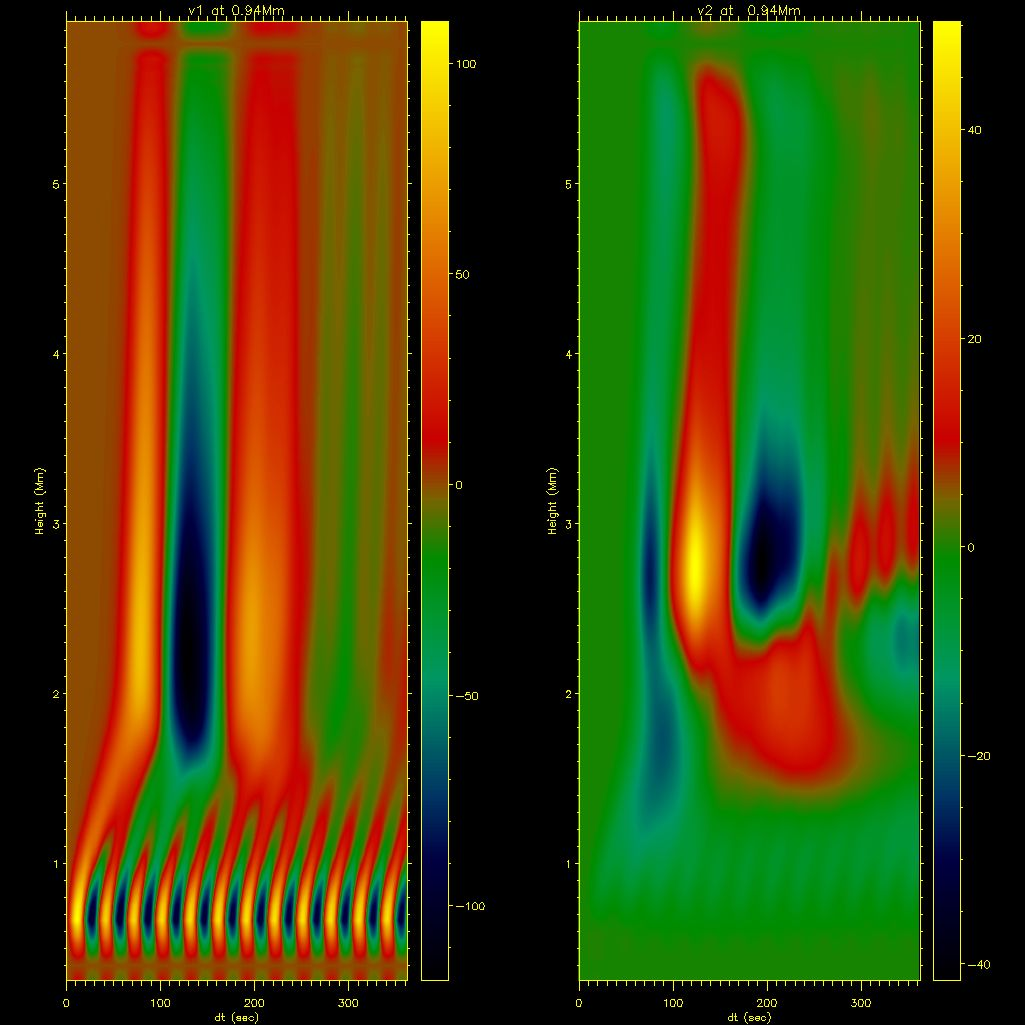
\includegraphics[scale=0.5]{images/pm30s_sindrv_n0_4b03d_dt.jpg}
%\caption{Three-dimensional snapshots of the evolution of Vz showing the development of the initial perturbation in the nonmagnetic equilibrium generated by the 30-second-period %driver (in ms−1) at the times (a) t = 112 seconds, (b) t = 216 seconds, (c) t = 244 seconds, and (d) t = 316 seconds. The z-axis corresponds to height measured in megameters and the x and y %horizontal axes are parallel to the solar surface. }
%\end{figure*}


%FIGURE 3 here caption:Distance time plot for fundamental model and 30s,180s and 300s driver period for the z component of the velocity for a vertical slice across the box  taken at 2Mm (shows  the profile of $v_{z}$ through the solar atmosphere for different time steps).\\

\begin{figure*}[h]\label{fig6_dt_30_180_300_0_vert_2Mm}
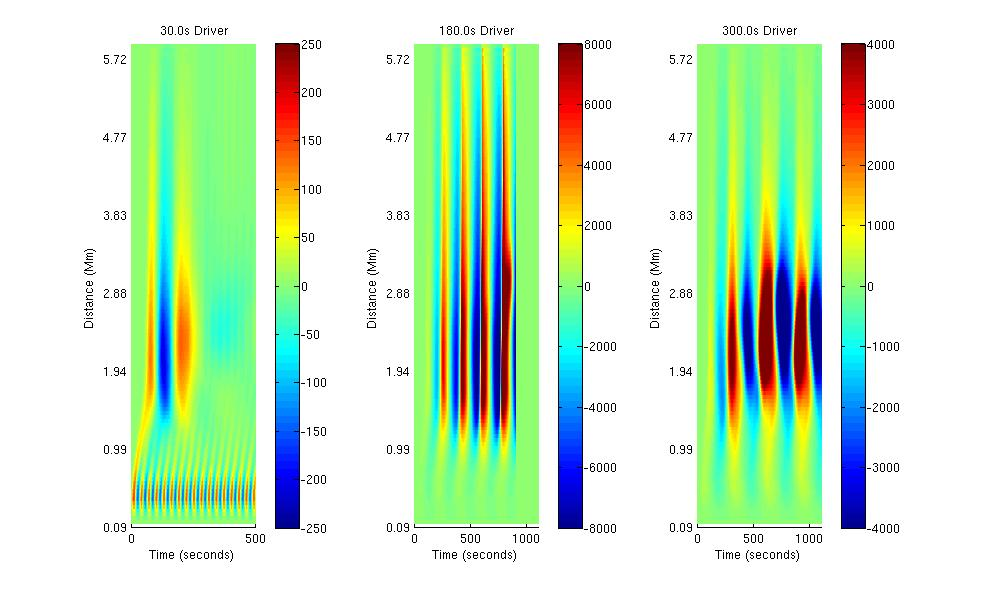
\includegraphics[scale=0.4]{images/fig4_dt_30_180_300_0_vert_2Mm.jpg}
\caption{Distance time plot for fundamental model and 30s,180s and 300s driver period for the z component of the velocity for a vertical slice across the box  taken at 2Mm and shows  the profile of $v_{z}$ through the solar atmosphere for different time steps. }
\end{figure*}


%FIGURE 4 here caption:Distance time plot for fundamental model and 30s,180s and 300s driver period for the z component of the velocity for a horizontal slice across the box  taken at 0.94Mm (shows  the profile of v_{z} across the simulation box at a given point in the solar chromosphere for different time steps). \\

\begin{figure*}[h]\label{fig7_dt_30_180_300_0_horiz_p94Mm}
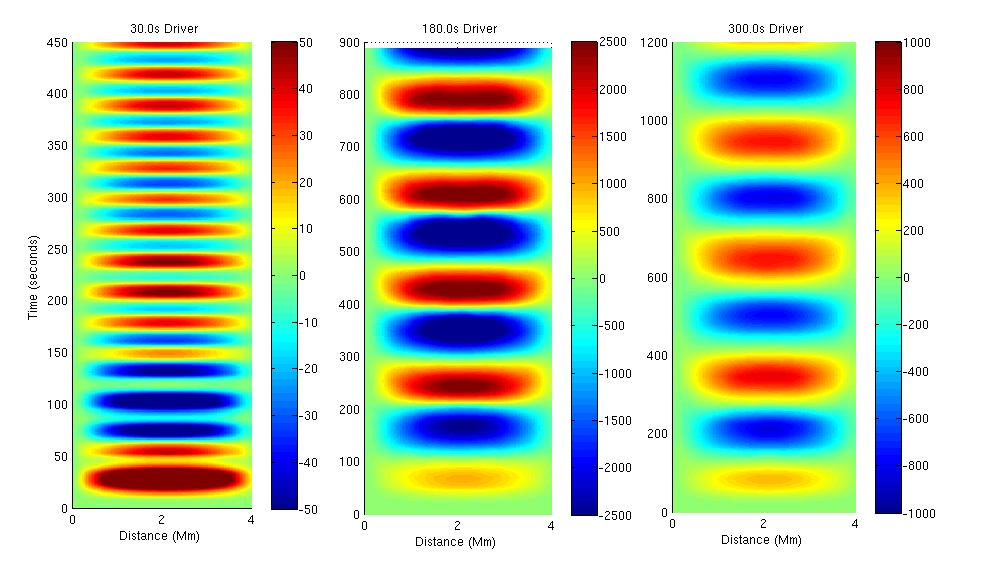
\includegraphics[scale=0.4]{images/fig5_dt_30_180_300_0_horiz_p94Mm.jpg}
\caption{Distance time plot for fundamental model and 30s,180s and 300s driver period for the z component of the velocity for a horizontal slice across the box  taken at 0.94Mm shows  the profile of $ v_{z}$ across the simulation box at a given point in the solar chromosphere for different time steps. }
\end{figure*}

%FIGURE 5 here caption:Distance time plot for fundamental model and 30s,180s and 300s driver period for the z component of the velocity for a horizontal slice across the box  taken at the transition zone (shows  the profile of $v_{z}$ across the simulation box at a height of 2Mm in the solar atmosphere for different time steps). \\

\begin{figure*}[h]\label{fig8_dt_30_180_300_0_horiz_2Mm}
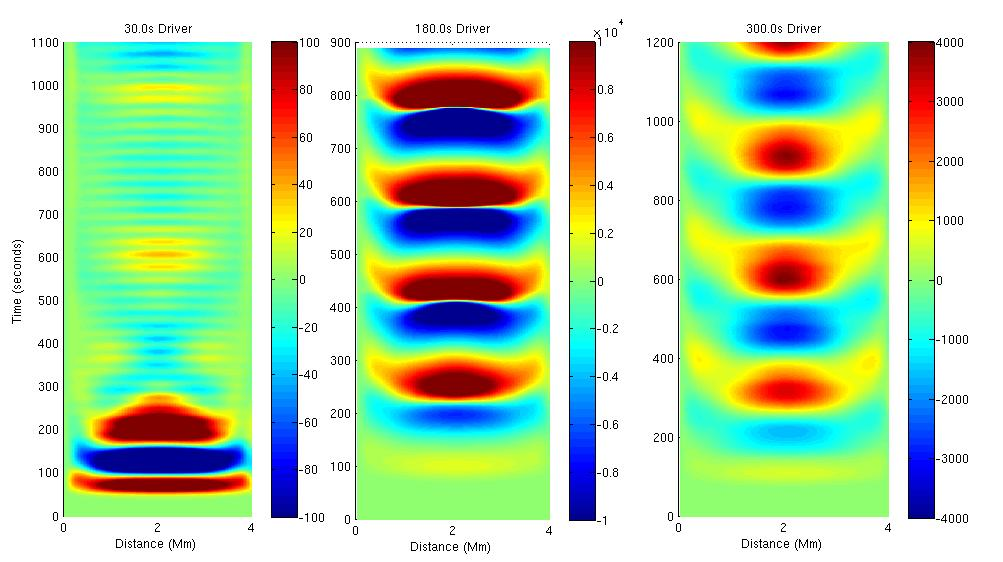
\includegraphics[scale=0.4]{images/fig6_dt_30_180_300_0_horiz_2Mm.jpg}
\caption{Distance time plot for fundamental model and 30s,180s and 300s driver period for the z component of the velocity for a horizontal slice across the box  taken at the transition zone shows  the profile of $v_{z}$ across the simulation box at a height of 2Mm in the solar atmosphere for different time steps. }
\end{figure*}


%FIGURE 6 here caption:Distance time plot for fundamental model and 30s,180s and 300s driver period for the z component of the velocity for a horizontal slice across the box  taken at 0.94Mm (shows  the profile of $v_{z}$ across the simulation box at a given point in the solar chromosphere for different time steps). \\

\begin{figure*}[h]\label{fig9_dt_30_180_300_0_horiz_4p2Mm}
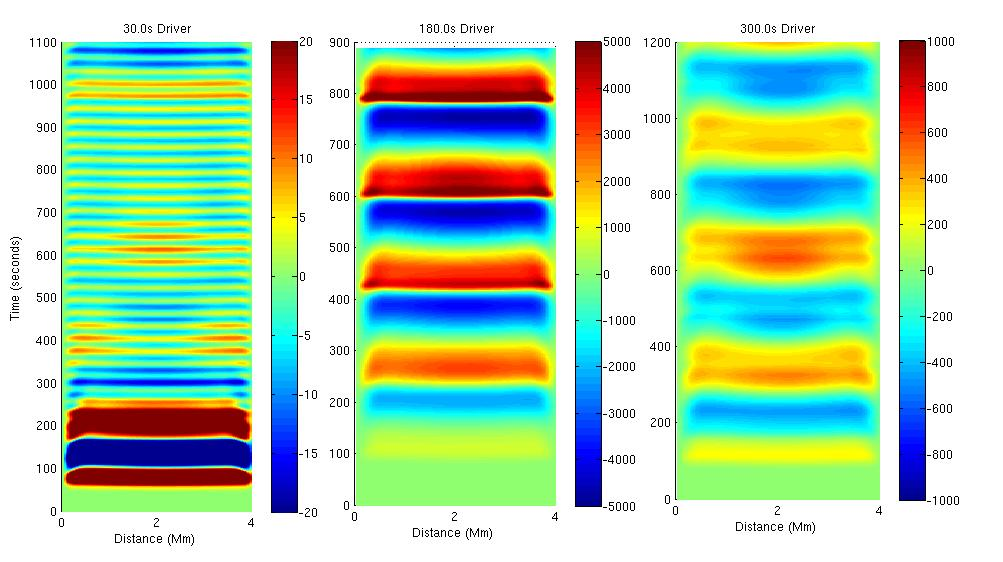
\includegraphics[scale=0.4]{images/fig7_dt_30_180_300_0_horiz_4p2Mm.jpg}
\caption{Distance time plot for fundamental model and 30s,180s and 300s driver period for the z component of the velocity for a horizontal slice across the box  taken at 4.2Mm shows  the profile of $v_{z}$ across the simulation box at a given point in the solar atmosphere for different time steps. }
\end{figure*}




















With the objective of characterising and understanding the nature of the frequencyy shifts of the excited modesWe consider a number of cases.

Since we want to investigate how wave energy propagation is influenced by the wave modes and frequencies, we compute the time averaged wave energy flux integrated over the cros-sectional area of the simulation box at different heights. The area of integration is perpendicular to the model z axis.

\begin{equation}\label{eqwaveenergyfluxintegral}
F_{int}= \frac{1}{t_{max}} \int_{0}^{t_{max}} \int         \bf{F_{wave}} \cdot d\bf{A}   dt   ,
\end{equation}

Where the wave energy flux $\bold{F_{wave}}$ is given by

\begin{equation}\label{eqwaveenergyflux}
\bf{F_{wave}}=\tilde{p}_{k} \bf{v}+\frac{1}{\mu_{0}}(\bf{B_{b}}\cdot \bf{\tilde{B}})\bf{v}-\frac{1}{\mu_{0}}(\bf{v}\cdot\bf{\tilde{B}})\bf{B_{b}}
\end{equation}

We have used the expression for the wave energy fluxused by 
 $\tilde{p}_{k}$ is the perturbed kinetic pressure given by \cite{Bogdan2003}

\begin{equation}\label{eqperturbpk}
\tilde{p}_{k}=(\gamma - 1)( \tilde{e}-{{(\tilde{\rho} +\rho_{b})\bf v }^{2}\over{2}}-  {{\bf \tilde{B}}^{2}\over{2}}-\bf{B_{b}} \cdot  \bf{\tilde{B}}).
\end{equation}




\begin{table*}
\centering
\begin{tabular}{c c c c }
\hline
Label   &  Density Profile & Gravity Enabled & Driver\\
\hline
B &  VALIIC & yes & single driver at photosphere & \\
\hline
C & VALIIC & no & single driver at photosphere &  \\
\hline
D & constant density & yes & single driver at photosphere &  \\
\hline
E & constant density & no & single driver at photosphere &  \\
\hline
F & constant density & no & two drivers at the photosphere and transition zone. &  \\
\hline
\end{tabular} 
\caption{Simulations Used to Characterise Oscillatory Motions Arising from the Surface Driver.}
\end{table*}






\section{Observations and Discussion}

The propagation of waves in a stratified atmosphere can be understood using linearised versions of the equation of continuity, momentum and energy. Such atmospheric waves of expansion have been considered for many years \cite{Lamb1932}.

Owing to the high gradients, partial reflection of acoustic waves at all frequencies is expected at the transition region. The transition region is the upper boundary of the chromospheric cavity, it has been previously suggested that this is the source of three-minute transition-region oscillations \cite{Leibacher1971}.

It is known that the propagation of acoustic waves in an unbounded medium is determined by a cut-off period. In a gravitationally stratified atmosphere acoustic waves can only propagate if the wave period is less than the cut off. It was shown that this frequency is a resonance, disturnaces with this frequency trigger a response. Waves with a period greater than the cut-off are evanescent.

The propagation of these acoustic wave modes in a gravitationally stratified atmosphere is determined by characterised cut off frequencies, theory predicts that waves will only propagate if the wave period is less than the local acoustic cut-off period in the atmosphere.

Following \cite{Taroyan2008} and solving the Klein-Gordon equation for the gravitationally stratified atmosphere \eqref{kgequation1} the cutoff for the atmosphere can be obtained \eqref{cutoff}
\begin{equation}\label{kgequation1}
\frac{\partial^2 Q}{\partial t^2} - c_s^2(z) \frac{\partial^2 Q}{\partial z^2} + \Omega^2(z)Q = 0 ,
\end{equation}

\begin{equation}\label{cutoff}
P_{c}(z)=\frac{   2\Lambda_0   }{ c_{s}(z)}   \sqrt{\frac{1}{1+2\frac{d\Lambda_0(z)}{dz}}} ,
\end{equation}

The pressure scale height for an atmosphere stratified by a uniform gravitational field
\begin{equation}\label{lambda0}
\Lambda_0(z)=\frac{p_0(z)}{g\rho_0(z)} ,
\end{equation}

The variation of the cutoff with solar atmospheric height is shown in figure \figref{cutofffrequency_fig4} which shows the cutoff period for the VALIIIc atmopshere and for an isothermal atmosphere. It is recognised from figure \figref{ cutofffrequency_fig4} that there is a number of distinct regions of propagation behaviour. For the photosphere near the temperature minimum  the cutoff period is 300s here it is expected that the 5 minutes modes are evanescent. In the chromosphere increases to a value greater than 300s, here the five minute modes can propagate. For the transition zone the cutoff drops to a value which goes down to 100s. In the corona it is seen that a much greater range of frequencies can propagate.

For the fundamental modes  illustrated in figure 4, 5 and 6 we observe that there is no significant structure at the transition zone. However, the 30s mode is particularly interesting detailed movies demonstrate the rapid expansion of the plume as it crosses the transition zone this is accompanied with an increase in the transverse velocity this observationi is true for both 180s, 30s and 300s driver scenarios. As the mode order is increased from $n=0$, to $n=1$ and then $n=2$ its is observed that transition region structuring becomes apparent and is more reminiscent of the observations of \cite{Malins2007B}.

For the fundamental modes with the 30s, 180s and 300s driver we have plotted distance-time diagrams of the z-component of the plasma velocity i.e. in the same direction as the driver and in the direction of increasing height through the solar atmosphere.  Figure
% \figref{dt_300_vert_x}
 shows the distance time plots for a vertical section through the simulation box, since this was a fundamental mode the section was taken through the middle of the simulation box. The plots show that the greatest amplitude arises in the transition region in particular for the 180s driver. Looking at the result for the 30s driver it is seen that the initial travelling response reaches a response at around 0.5Mm corresponding to a cut-off of 200s. The maximum amplitude is coherent with the maximum occuring at the same frequency as that of the driver. For the first 70 periods maxima appear in the transition zone. It appears that the transition zone is essentially a source of excitation with freuency lower than that of the driver, however, at longer time periods these motions occur with reduced amplitude but with the same period as the driver. For the180s and 300s drivers it is observed that the amplitude in the transition zone is larger than that for the 30s driver by a factor of upto 20. For the 30,180 and 300s case we observe the travelling wave in the Chromosphere and a stationary wave in the solar Corona. Although the 180s mode shows the greatest excitation both the 180s and 300s drivers become evanescent due the the cut-off for the upper atmosphere. Figure  shows the distance time plot for a horizontal section taken at a height of 0.94Mm, i.e. through the Chromosphere. The travelling modes in these plots propagate as plane modes with a frequecy consistent with that of the driver. The greatest intensity is observed for the 180s driver. Propagation for the transition zone shown in figure  shows the most powerful response for the 180s driver followed by the 300s driver. The response for the 30s driver decays rapidly after the first ten cycles. As we move into the Corona there is further attenuation with the greatest signal reduction for the 30s driver.

The distance-time plots  for horizontal sections at an atmospheric height of 4.2Mm are a clear indication of the propagation of waves across the transition zone for the case of the 30s driver it can be seen that  the propagation is cut-off after the first 270s of the simulation. All three driver cases indicate a peak with a width of around 90s this peak exhibits a degree of splitting which is most clear for the 300s driver.  This effect may be attributable to the superposition of waves reflected from the boundaries of the chromosphere.











%FIGURE 7 here caption:Distance time plot for fundamental model with 300s period for the z  component of the velocity. x-direction\\

\begin{figure*}[h]
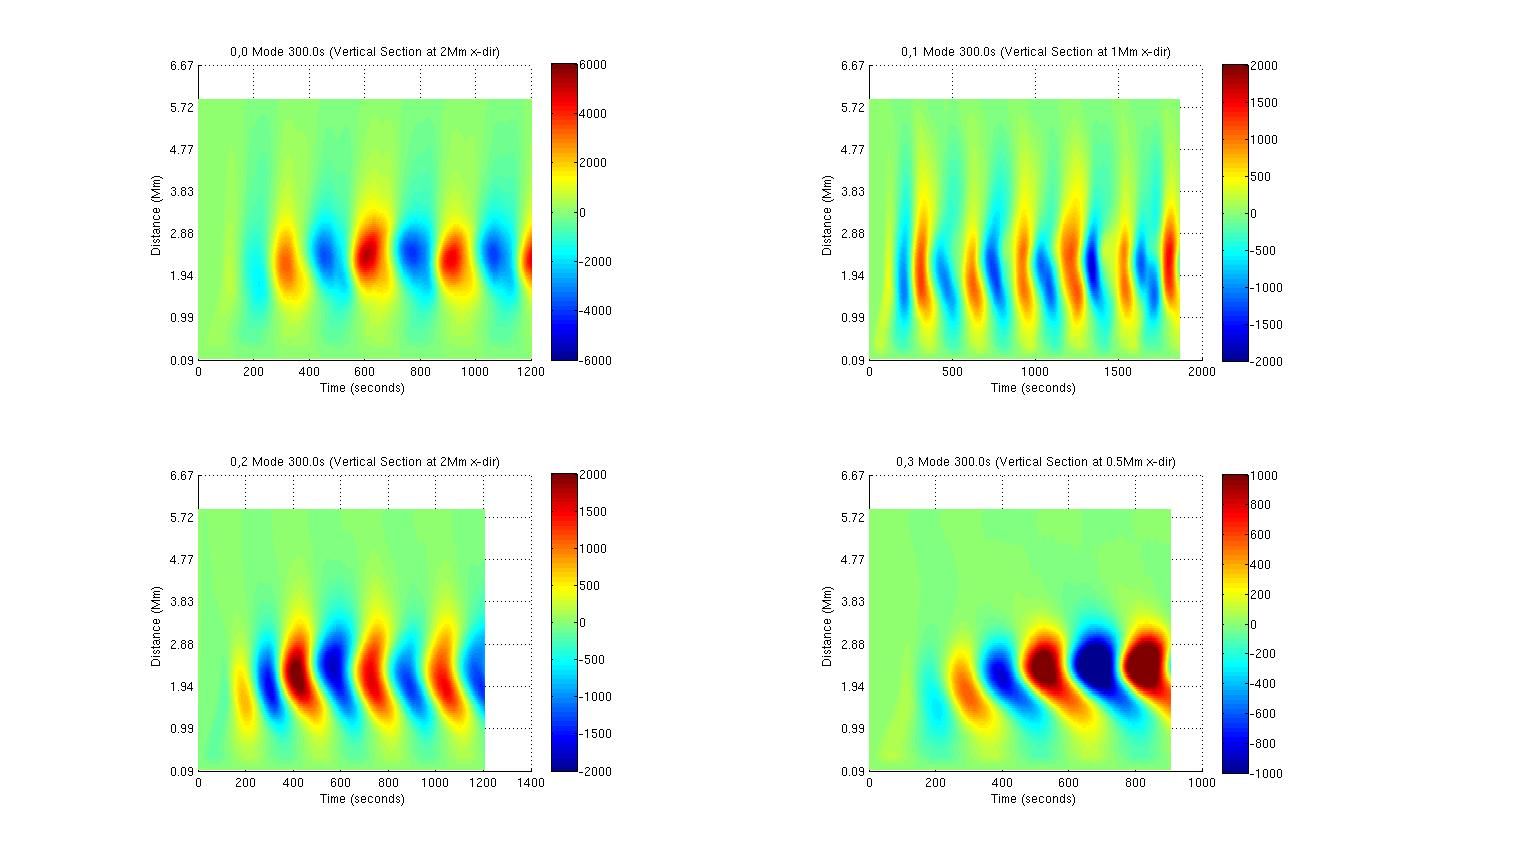
\includegraphics[scale=0.3]{imagesn/dt_300_vert_x.jpg}
\caption{Distance time plot for fundamental model with 300s period for the z component of the velocity. x-direction }
\label{dt_300_vert_x}
\end{figure*}

%FIGURE 8 here caption:Distance time plot for fundamental model with 180s period for the z  component of the velocity. x-direction\\

\begin{figure*}[h]
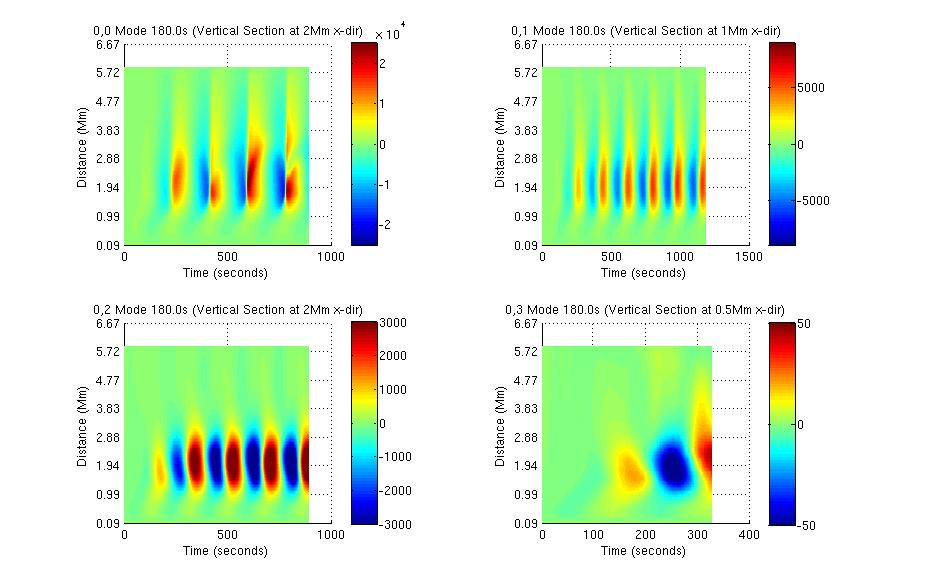
\includegraphics[scale=0.45]{imagesn/dt_180_vert_x.jpg}
\caption{Distance time plot for fundamental model with 180s period for the z component of the velocity.  x-direction}
\end{figure*}


%FIGURE 9 here caption:Distance time plot for fundamental model with 300s period for the z  component of the velocity. y-direction\\

\begin{figure*}[h]
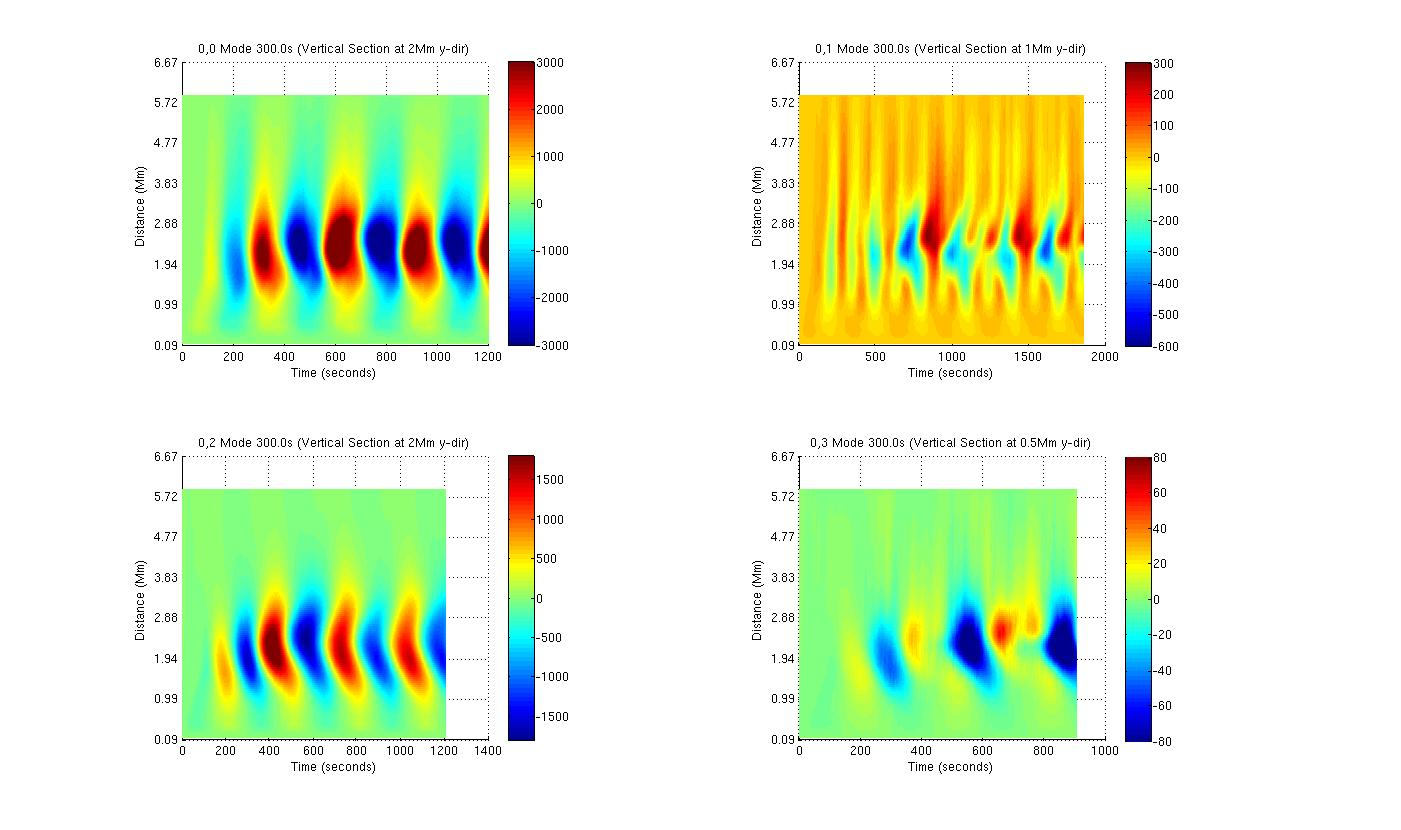
\includegraphics[scale=0.3]{imagesn/dt_300_vert_y.jpg}
\caption{Distance time plot for fundamental model with 300s period for the z component of the velocity. y-direction }
\end{figure*}

%FIGURE 10 here caption:Distance time plot for fundamental model with 180s period for the z  component of the velocity. y-direction\\

\begin{figure*}[h]
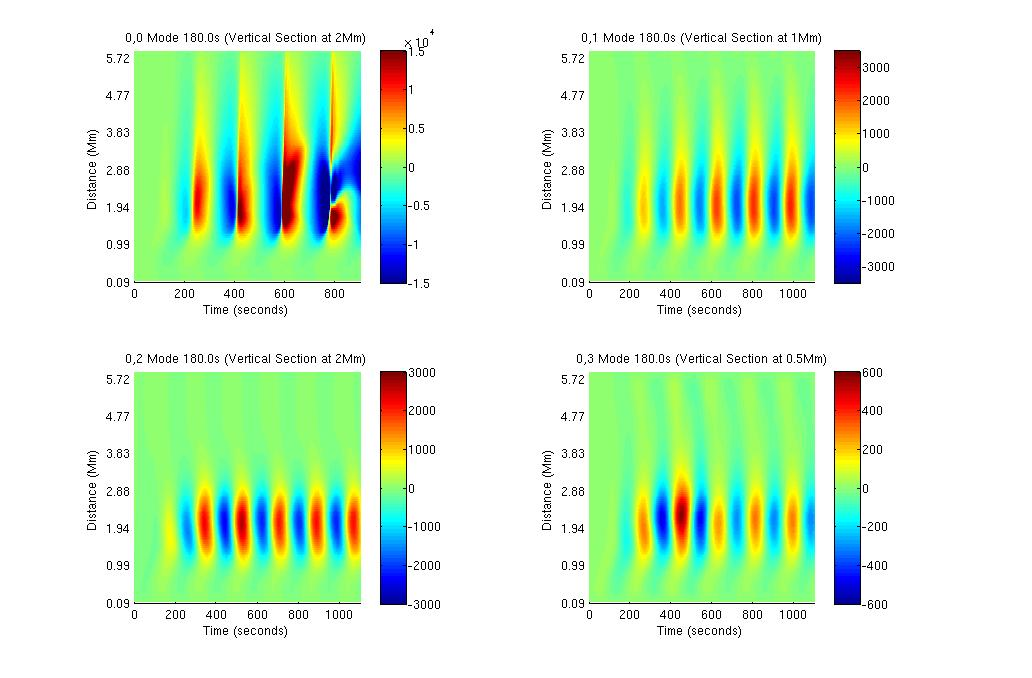
\includegraphics[scale=0.3]{imagesn/dt_180_vert_y.jpg}
\caption{Distance time plot for fundamental model with 180s period for the z component of the velocity.  y-direction}
\end{figure*}



%FIGURE 11 here caption:Distance time plot for modes with 300s period Horizontal Section through the Chromosphere (at 1Mm) for the z  component of the velocity. x-direction\\
\begin{figure*}[h]
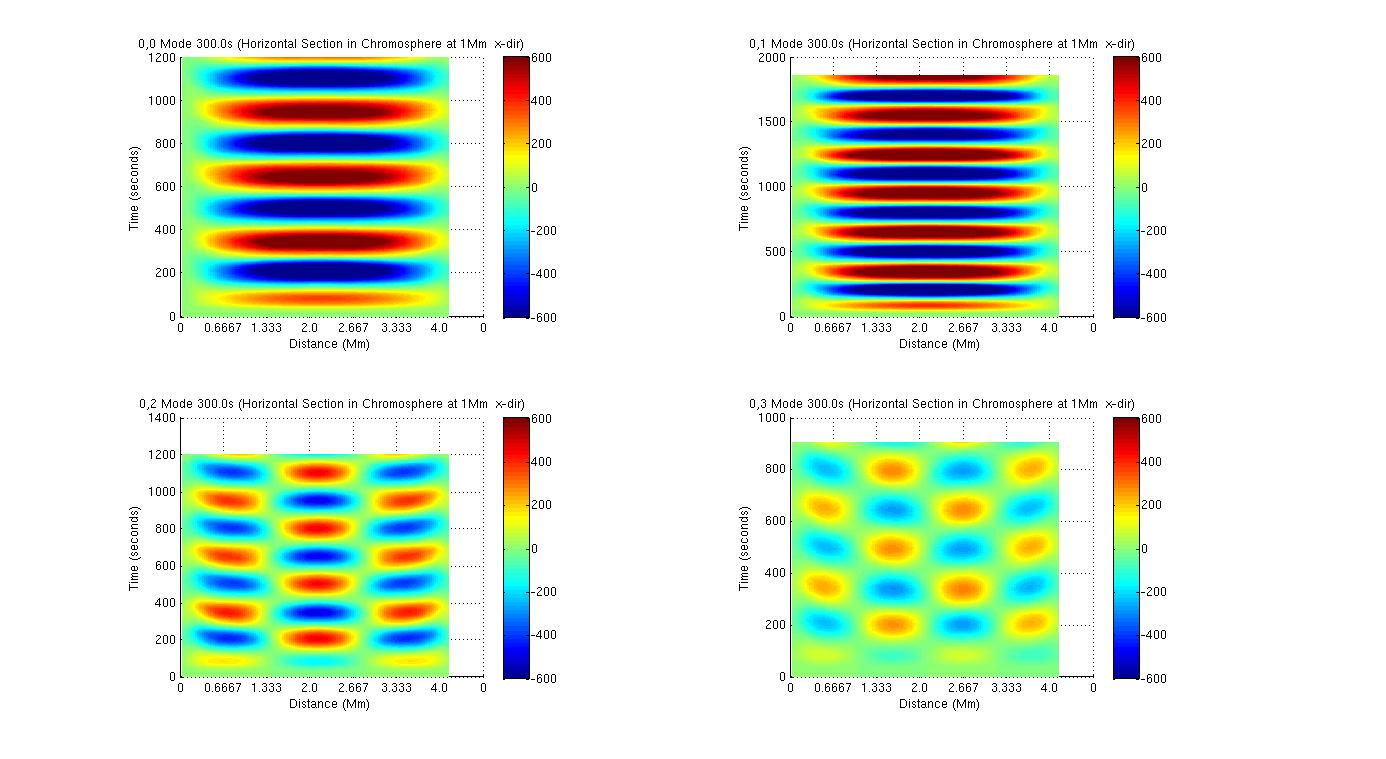
\includegraphics[scale=0.3]{imagesn/dt_300_0_0_hor_x_1Mm.jpg}
\caption{Distance time plot for modes with 300s period Horizontal Section through the Chromosphere (at 1Mm) for the z  component of the velocity. x-direction}
\end{figure*}

%FIGURE 12 here caption:Distance time plot for modes with 300s period Horizontal Section through the Transition Region (at 2.06Mm) for the z  component of the velocity. x-direction\\
\begin{figure*}[h]
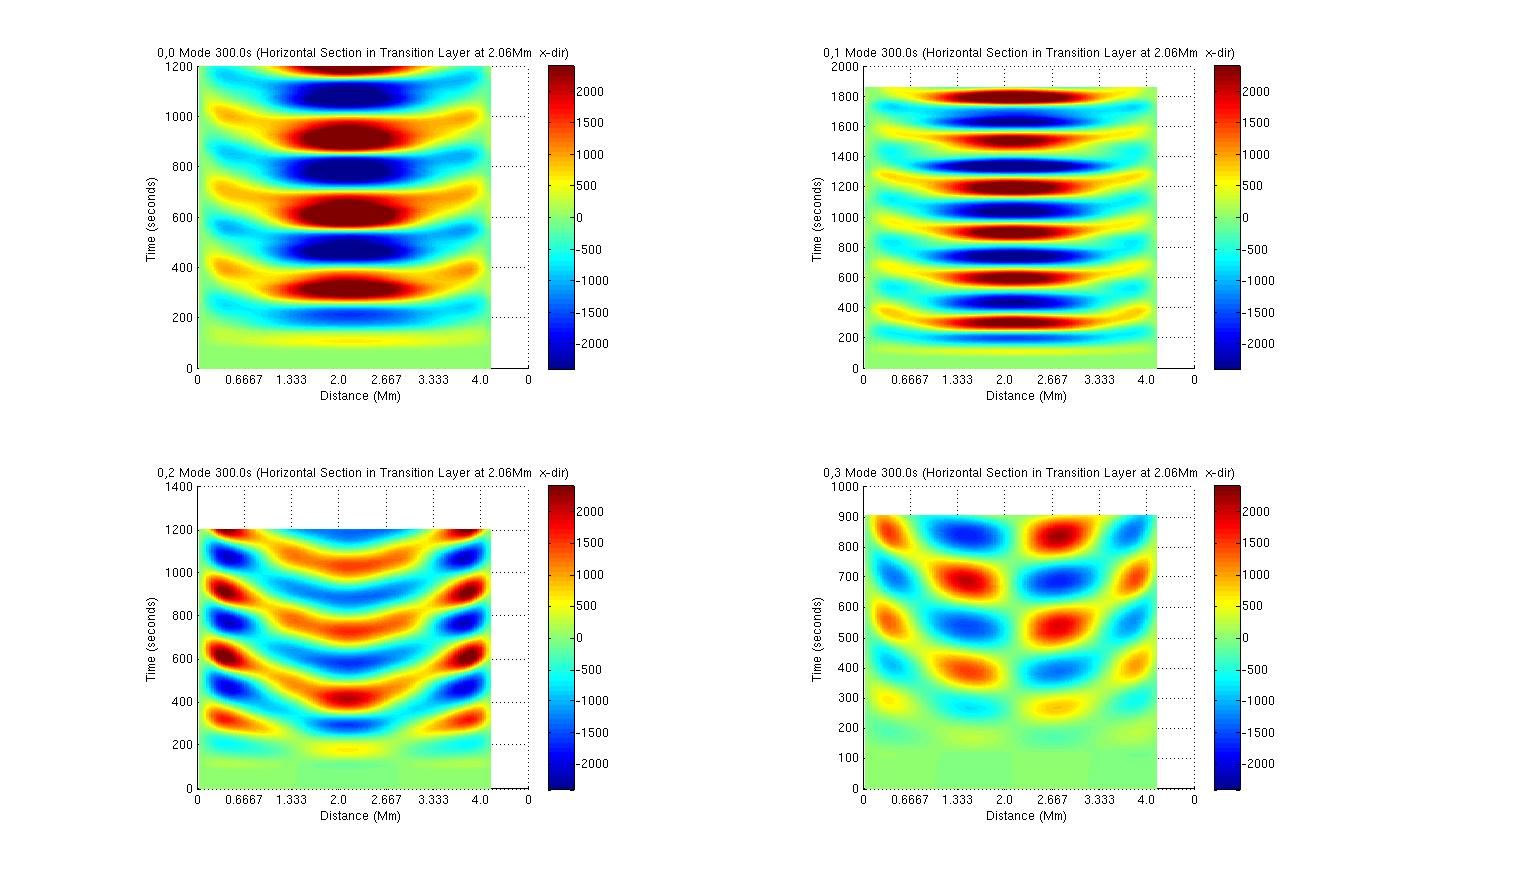
\includegraphics[scale=0.3]{imagesn/dt_300_hor_x_2p06Mm.jpg}
\caption{Distance time plot for modes with 300s period Horizontal Section through the Transition Region (at 2.06Mm) for the z  component of the velocity. x-direction}
\end{figure*}

%FIGURE 13 here caption:Distance time plot for modes with 300s period Horizontal Section through the Transition Region (at 4.3Mm) for the z  component of the velocity. x-direction\\
\begin{figure*}[h]
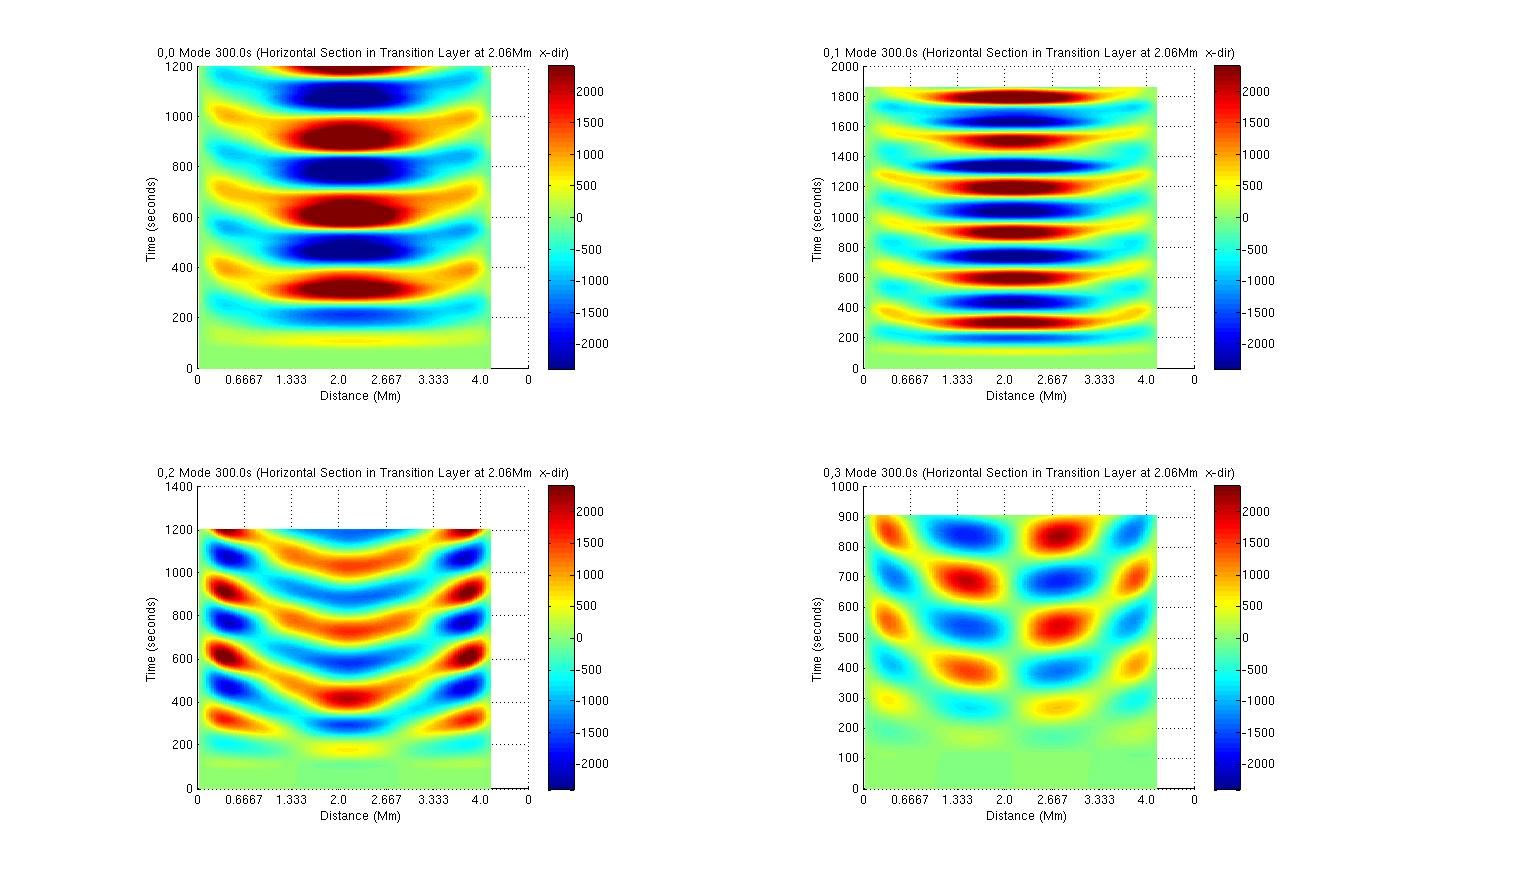
\includegraphics[scale=0.3]{imagesn/dt_300_hor_x_2p06Mm.jpg}
\caption{Distance time plot for modes with 300s period Horizontal Section through the Solar Corona (at 4.3Mm) for the z  component of the velocity. x-direction}
\end{figure*}


%FIGURE 14 here caption:Distance time plot for modes with 180s period Horizontal Section through the Chromosphere (at 1Mm) for the z  component of the velocity. x-direction\\
\begin{figure*}[h]
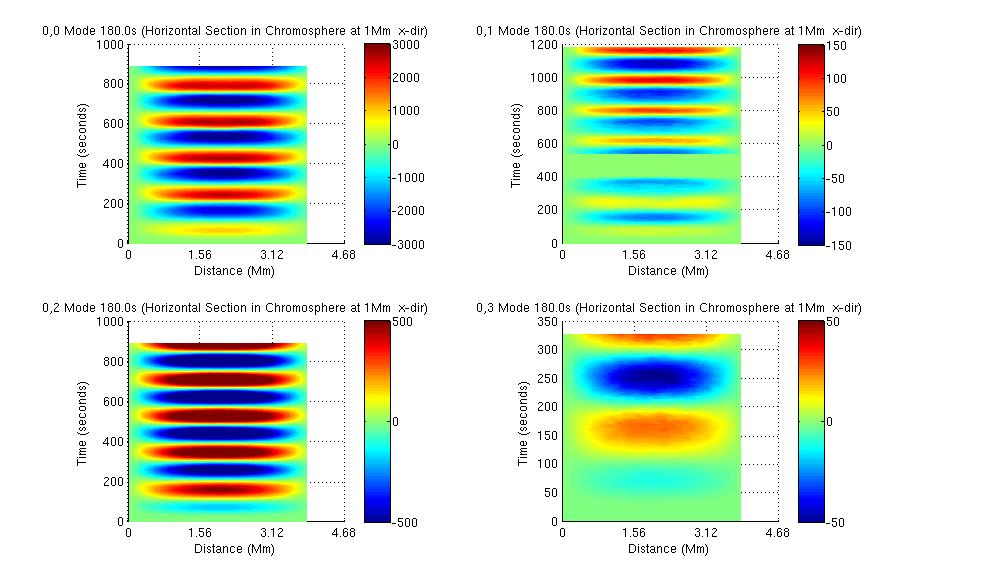
\includegraphics[scale=0.45]{imagesn/dt_180_horiz_x_1Mm.jpg}
\caption{Distance time plot for modes with 180s period Horizontal Section through the Chromosphere (at 1Mm) for the z  component of the velocity. x-direction}
\end{figure*}

%FIGURE 15 here caption:Distance time plot for modes with 180s period Horizontal Section through the Transition Region (at 2.06Mm) for the z  component of the velocity. x-direction\\
\begin{figure*}[h]
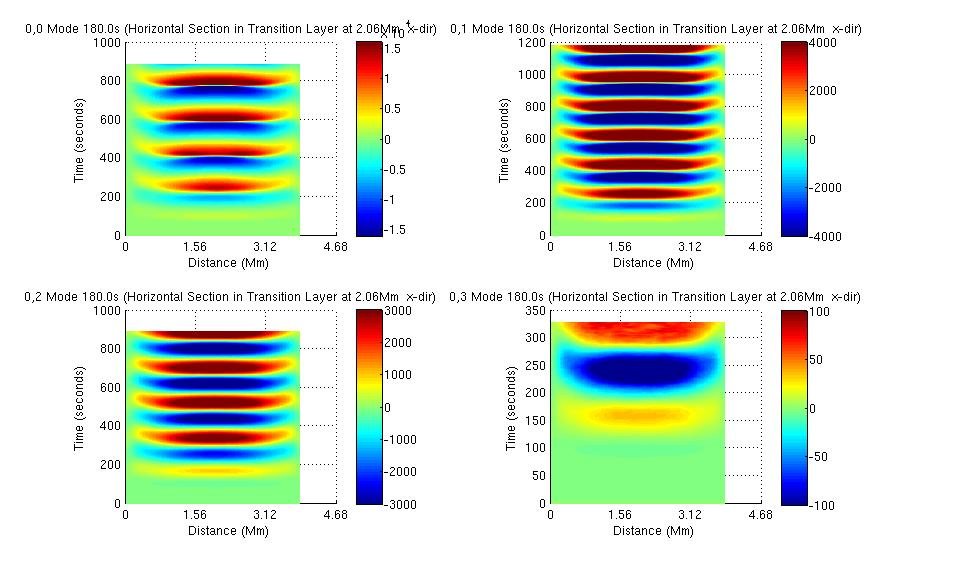
\includegraphics[scale=0.5]{imagesn/dt_180_horiz_x_2p06Mm.jpg}
\caption{Distance time plot for modes with 180s period Horizontal Section through the Transition Region (at 2.06Mm) for the z  component of the velocity. x-direction}
\end{figure*}

%FIGURE 16 here caption:Distance time plot for modes with 180s period Horizontal Section through the Transition Region (at 4.3Mm) for the z  component of the velocity. x-direction\\
\begin{figure*}[h]
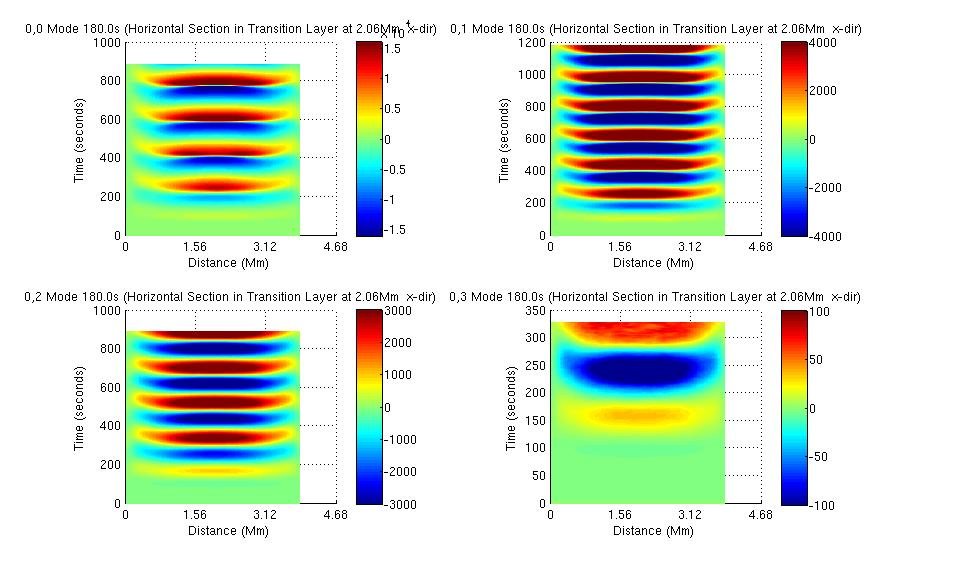
\includegraphics[scale=0.5]{imagesn/dt_180_horiz_x_2p06Mm.jpg}
\caption{Distance time plot for modes with 180s period Horizontal Section through the Solar Corona (at 4.3Mm) for the z  component of the velocity. x-direction}
\end{figure*}

Using equation \eqref{eqwaveenergyfluxintegral} we compute the energy flux integral for the range of driver frequencies, modes and at different atmospheric heights. Figure 17
shows the variation of the energy flux ratio, we compute the ratio of the energy flux at a height of 5.5Mm to the driver energy ratio.  The figure shows the energy ratios for the different modes. Fitting  the  data for the (0,0) mode against the power law shown in equation \eqref{energyfluxpowerlaw} gives the values shown in table 12. The powerlaw values are in agreement the values obtained from the observational results of Ireland \cite{Ireland2014} distinguishing a flat power spectrum for high frequencies and a power spectrum for low frequencies.

\begin{equation}\label{energyfluxpowerlaw}
P(z)= aT^{b}+c ,
\end{equation}


\begin{table*}
\centering
\begin{tabular}{c c c c }
\hline
   &  Fitted Values & Ireland (171{\AA}) & Ireland (193{\AA}) \\
\hline
a & -6.199x$10^{-9}$ &  $10^{0.57}$ & $10^{-0.1}$ \\
\hline
b & 1.762 & 1.72 & 2.2 \\
\hline
c & 0.002872 & $10^{-3}$ & $10^{-3.52}$ \\
\hline
\end{tabular} 
\caption{ Power law coefficients for relationship between power and time-period of atmospheric oscillation.}
\end{table*}

The results tables show the values of the energy flux from the simulations at different heights. All the modes for the driver periods 180s and 300s are shown as a bar chart in figure 18 and figure 19. For both the 180s and 300s drivers it can be seen that the even modes make the strongest contribution in the corona. The results plotted in figure 20 show the ratio of the Energy flux for models delivering the same quantity of energy to the energy flux for models where the driver amplitude is kept fixed. With the exception of the fundamental mode the ratios appear to be constant for all frequencies suggesting the possibility of using the scaling relation to compute the enrgy flux for differenet frequencies and modes.  



\begin{table*}
\centering
\begin{tabular}{c c c c c }
\hline
   &  1Mm & 2Mm & 4Mm & 5.5Mm \\
\hline
30 &  0.0133 & 1.7275x$10^{-4}$ & 1.0561x$10^{-4}$ & 5.5399x$10^{-5}$ \\
\hline
300 & 0.2607 & 0.008144 & 0.002176 &  0.001119 \\
\hline
180 & 0.7227 & 0.047895 & 0.019831 &  0.010365 \\
\hline
435.1 & 1.9415 & 0.043601 & 0.005944 & 0.003147  \\
\hline
179.98 & 1.6450 & 0.004502 & 0.002600&  0.001366 \\ 
\hline
282.84 & 0.1986 & 0.004007 & 0.001845 &  9.7821x$10^{-4}$ \\
\hline
\end{tabular} 
\caption{ (00) mode energy ratio.}
\end{table*}




\begin{table*}
\centering
\begin{tabular}{c c c c c }
\hline
   &  1Mm & 2Mm & 4Mm & 5.5Mm \\
\hline
30 &  0.0065 & 1.751x$10^{-5}$ &  1.2579x$10^{-6}$ & 4.6820x$10^{-7}$ \\
\hline
300 & 0.1001 & 8.796x$10^{-4}$ &  4.1494x$10^{-6}$ &  1.3059x$10^{-6}$ \\
\hline
180 & 0.1543 &  5.8381x$10^{-4}$ &  3.2715x$10^{-5}$ &  1.1343 x$10^{-5}$ \\
\hline
307.1 & 0.0982 & 0.001 & 4.1351x$10^{-6}$ & 1.3380 x$10^{-6}$  \\
\hline
127.27 & 0.0829 &  4.3190x$10^{-4}$ &  5.1387x$10^{-5}$ & 2.0397 x$10^{-5}$ \\ 
\hline
200.0 & 0.1126 &  4.4180x$10^{-4}$ &  2.0186x$10^{-5}$ & 6.3062 x$10^{-6}$ \\
\hline
\end{tabular} 
\caption{ (01) mode energy ratio.}
\end{table*}







\begin{table*}
\centering
\begin{tabular}{c c c c c }
\hline
   &  1Mm & 2Mm & 4Mm & 5.5Mm \\
\hline
30 &  0.0024 & 7.2158 x$10^{-6}$ & 1.0651x$10^{-6}$ & 7.6079x$10^{-7}$\\
\hline
300 & 0.0578 & 4.9604 x$10^{-4}$ & 5.5618x$10^{-6}$ & 4.1907x$10^{-6}$\\
\hline
180 & 0.0687 & 3.5547 x$10^{-4}$ & 6.0675x$10^{-5}$ & 4.1492 x$10^{-5}$\\
\hline
205.1 & 0.3135 & 0.0015 &1.6520x$10^{-4}$ & 1.1272x$10^{-4}$\\
\hline
84.84 & 0.0206 &5.8903 x$10^{-5}$1.6520 x$10^{-5}$ & 1.1890 x$10^{-5}$\\
\hline
133.33 & 0.0497 & 1.9731x$10^{-4}$7.9834 x$10^{-5}$ & 5.6267 x$10^{-5}$\\
\hline
\end{tabular} 
\caption{ (02) mode energy ratio.}
\end{table*}




\begin{table*}
\centering
\begin{tabular}{c c c c c }
\hline
   &  1Mm & 2Mm & 4Mm & 5.5Mm \\
\hline
30 &  0.0101 &  4.2736x$10^{-5}$ & 6.3291x$10^{-7}$ & 3.7786x$10^{-7}$\\
\hline
300 & 0.0359 & 3.8929x$10^{-4}$ & 3.2621x$10^{-7}$ & 2.1259x$10^{-7}$\\
\hline
180 & 0.0351 &1.3948x$10^{-4}$ & 3.1342x$10^{-6}$ & 1.8205x$10^{-6}$\\
\hline
153.8 & 0.0313 & 1.1043x$10^{-4}$ & 3.8071x$10^{-6}$ & 2.1034x$10^{-6}$\\
\hline
63.63 & 0.0051 & 9.8989x$10^{-6}$ & 7.0207x$10^{-7}$ & 4.0621x$10^{-7}$\\
\hline
100.0 & 0.0151 & 3.0678x$10^{-5}$ & 2.8527x$10^{-6}$ & 1.6707x$10^{-6}$\\
\hline
\end{tabular} 
\caption{ (03) mode energy ratio .}
\end{table*}





\begin{table*}
\centering
\begin{tabular}{c c c c c }
\hline
   &  1Mm & 2Mm & 4Mm & 5.5Mm \\
\hline
(0,0) &  0.7227 & 0.0479 & 0.0198 & 0.0104 \\
\hline
(0,1) & 0.1543 & 0.0006 & 3.2715x$10^{-5}$ &  1.1343x$10^{-5}$\\
\hline
(0,2) & 0.0687 & 0.0004 & 6.0675x$10^{-5}$ &  4.1492x$10^{-5}$\\
\hline
(0,3) & 0.0351 & 0.0001 & 3.1342x$10^{-6}$ & 1.8205 x$10^{-6}$\\
\hline
(1,1) & 0.4072 & 0.0011 & 4.5311x$10^{-6}$ &  5.5495x$10^{-7}$\\
\hline
(1,2) & 0.3331 & 0.0012 & 3.0728x$10^{-6}$ &  1.3055x$10^{-6}$\\
\hline
(1,3) & 0.2961 & 0.0011 & 4.8733x$10^{-7}$ &  3.4760x$10^{-7}$\\
\hline
(2,2) & 0.3054 & 0.0011 & 1.5844x$10^{-5}$ &  1.7622x$10^{-5}$\\
\hline
(2,3) & 0.2732 & 0.0008 & 2.1443x$10^{-6}$ &  1.7045x$10^{-6}$\\
\hline
(3,3) & 0.2205 & 0.0006 & 1.9711x$10^{-7}$ &  2.6756x$10^{-7}$\\
\hline
\end{tabular} 
\caption{ 180s driver energy ratio. }
\end{table*}





\begin{table*}
\centering
\begin{tabular}{c c c c c }
\hline
   &  1Mm & 2Mm & 4Mm & 5.5Mm \\
\hline
(0,0) &  0.2607 & 0.0081 & 2.2x$10^{-3}$ &  1.1x$10^{-3}$\\
\hline
(0,1) & 0.1001 & 0.0009 & 4.1494x$10^{-6}$ &  1.3059x$10^{-6}$\\
\hline
(0,2) & 0.0578 & 0.0005 & 5.5618x$10^{-6}$ &  4.1907x$10^{-6}$\\
\hline
(0,3) & 0.0359 & 0.0004 &3.2621x$10^{-7}$ &  2.1259x$10^{-7}$\\
\hline
(1,1) & 0.2267 & 0.0016 & 9.9329x$10^{-7}$ &  1.0749x$10^{-7}$\\
\hline
(1,2) & 0.2535 & 0.0016 & 8.2058x$10^{-7}$ &  2.8814x$10^{-7}$\\
\hline
(1,3) & 0.2692 & 0.0023 & 2.1995x$10^{-7}$ &  9.0161x$10^{-8}$\\
\hline
(2,2) & 0.2625 & 0.0021 & 1.4846x$10^{-6}$ &  1.7399x$10^{-6}$\\
\hline
(2,3) & 0.2328 & 0.0017 & 2.4839x$10^{-7}$ &  2.0699x$10^{-7}$\\
\hline
(3,3) & 0.2036 & 0.0012 & 7.2069x$10^{-8}$ &  4.944x$10^{-8}$\\
\hline
\end{tabular} 
\caption{ 300s driver energy ratio percentage. }
\end{table*}


\clearpage

%FIGURE 17 here caption:Variation of Energy Flux Ratio with the Driver Energy at a Height of 5.5Mm for a Solar Atmosphere Excited with a p-Mode Driver Located at a Height of 50km\\
\begin{figure*}[t]
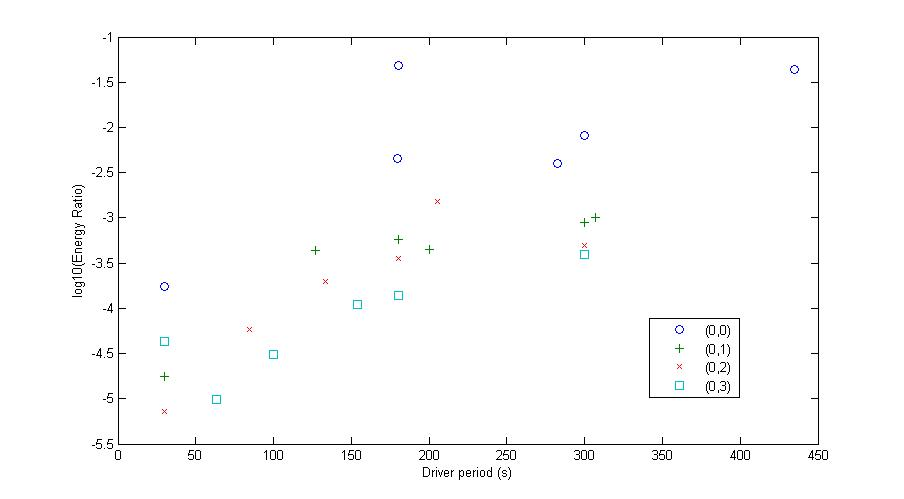
\includegraphics[scale=0.4]{imagesn/ratio_varoverdrve_eflux_vperiod_for modes_5p5Mm.jpg}
\caption{Variation of Energy Flux Ratio with the Driver Energy at a Height of 5.5Mm for a Solar Atmosphere Excited with a p-Mode Driver Located at a Height of 50km}
\end{figure*}


\clearpage

%FIGURE 18 here caption:Variation of Energy Flux Ratio at a Height of 5.5Mm for a Solar Atmosphere Excited with a 180s p-Mode Driver Located at a Height of 50km\\
\begin{figure*}[h]
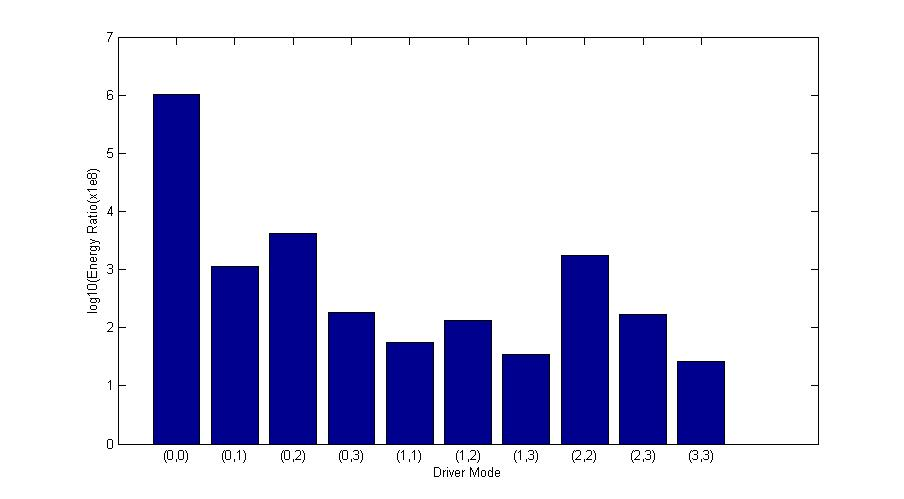
\includegraphics[scale=0.5]{imagesn/ratio_varoverdrve_eflux_vperiod_forallmodes_180s_5p5Mm.jpg}
\caption{Variation of Energy Flux Ratio at a Height of 5.5Mm for a Solar Atmosphere Excited with a 180s p-Mode Driver Located at a Height of 50km}
\end{figure*}



%FIGURE 19 here caption:Variation of Energy Flux Ratio at a Height of 5.5Mm for a Solar Atmosphere Excited with a 180s p-Mode Driver Located at a Height of 50km\\
\begin{figure*}[h]
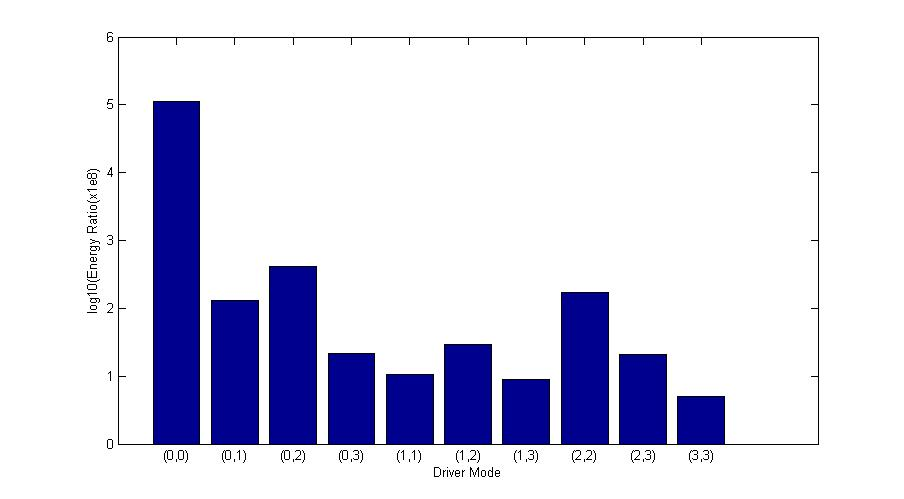
\includegraphics[scale=0.5]{imagesn/ratio_varoverdrve_eflux_vperiod_forallmodes_300s_5p5Mm.jpg}
\caption{Variation of Energy Flux Ratio at a Height of 5.5Mm for a Solar Atmosphere Excited with a 300s p-Mode Driver Located at a Height of 50km}
\end{figure*}

\clearpage


%FIGURE 20 here caption:Variation of Energy Flux Ratio at a Height of 5.5Mm for a Solar Atmosphere Excited with a p-Mode Driver Located at a Height of 50km\\
\begin{figure*}[h]
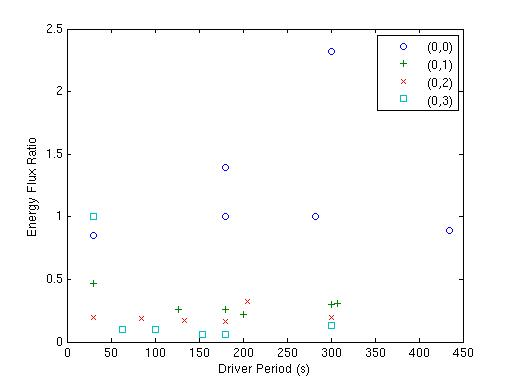
\includegraphics[scale=0.6]{imagesn/ratio_varoverconst_eflux_vperiod_for modes_5p5Mm.jpg}
\caption{Variation of Energy Flux Ratio at a Height of 5.5Mm for a Solar Atmosphere Excited with a p-Mode Driver Located at a Height of 50km}
\end{figure*}



%______________________________________________________________


%______________________________________________________________

\section{Conclusions}

Our results support the notion that solar global oscillations are a driver for a range of global dynamical phenomena resulting in atmospheric and chr0mospheric oscillations which contribute to the propagation of energy into the solar atmosphere.  Global dynamical phenomena arise from a range of sources including solar global oscillations, turbulent motions from convective cells and nano flares giving the possibility of continuous reconnection events.
   \begin{enumerate}
      \item The  consistency of the frequency dependence of the energy flux for our numerical simulations and powel flux measurements obtained from SDO supports the use of numerical simulations for modelling the excitations driven by solar global oscillations for the quiet sun.
      \item Agreement between the energy flux predictions of our numerical simulations and the the two layer Klein-Gordon model supports
      \item Energy propgation into the atmosphere occurs for a range of frequencies and may explain observed intensity oscillations for periods greater than the well known 3 minute and 5 minute oscillations.  
      \item Energy flux propagation into the solar corona is strongly dependent on the wave modes
   \end{enumerate}

\begin{acknowledgements}
RE acknowledges M. K\'eray for patient encouragement and is also grateful to NSF, Hungary (OTKA, Ref. No. K83133). 
The authors thank the Science and Technology Facilities Council (STFC), UK for the support they received. We acknowledge Corporate Information and Computing Services at The University of Sheffield for the provision of the High Performance Computing Service.
\end{acknowledgements}


\section{References}
\bibliographystyle{elsarticle-num-names}
%\bibliographystyle{unsrt}
\bibliography{eigenmodes_2016_v1}
%\begin{thebibliography}{XXX}
%\end{thebibliography}





\end{document}
